\chapter{Analyzing Optimizer Behavior}

This chapter provides a brief overview of some of the tools provided in Mesquite for assisting with the analysis and visualization of the Mesquite optimization process.  The tools discussed in this section can be used to provide additional output.	 External tools such as Paraview, VisIt, or GNU Plot must be used to visualize the data.

\section{Assessing Quality}

  The QualityAssessor class provides a summary of the mesh quality. It can be used with Non Target-paradigm metrics (QualityMetric classes) as well as Target-paradigm metrics (TMetric classes). For simplicity, the following discussion refers to the QualityMetrics classes but the concepts apply to the TMetric classes as well.	The QualityAssessor class can be used in a direct fashion as shown in the example below or via the InstructionQueue class as described in Section \ref{sec:tutDetailedAPI}.  An instance of the QualityMetric class can be specified for the QualityAssessor instance at creation to be used to assess the mesh quality.  Additional QualityMetric instances can be created using the Assessor class and by adding them to the QualityAssessor instance via the "add\_quality\_assessment" method. If no QualityMetrics are specified, the only assessment that will be performed is a simple count of inverted elements. One or more instances of the QualityAssessor class may be inserted in the InstructionQueue at any point to print a summary of the mesh quality at that time during the optimization.

\subsection{Stopping Assessment}

A stopping assessment can be specified for each QualityAssessor instance.  The "stopping assessment" directs the assessment code calculate a value using the power mean data to use that value as the return value for the loop\_over\_mesh call.  If no power mean is specified for a QualityAssessor instance, a simple average of all metric values calculated during the assessment is returned from  loop\_over\_mesh.  Only one stopping assessment with its associated power mean can be specified for a particular QualityAssessor instance.  There are three different ways to specify a stopping assessment: when the QualityAssessor instance is created using a constructor, when a quality assessment is added via the add\_quality\_assessment () method, and directly with the set\_stopping\_assessment() method.  Since only one stopping assessment can be defined for a each instance of QualityAssessor, the last action that causes the stopping assessment to be set will be the one used for the assessment no matter how many metrics have been included.

\subsection{Using the Quality Assessor}

  The QualityAssessor class provides a number of constructors.	Each allows the specification of a different set parameters to control the quality assessment.	The parameters are described below including default values, if any. Note that all parameters are not used in each constructor.

\label{QA_params}
Parameters used by QualityAssesor constructors:
\begin{description}
\item[metric:]	 QualityMetric to register for use in assessing mesh quality.  Will also be used in the setting of the stopping assessment.

\item[histogram\_intervals:]   If non-zero, a histogram of quality metric values composed of the specified number of intervals will be generated.  Default is zero.
\item[power\_mean:] If non-zero, in addition to the normal summary statistics for the quality metric, an additional general power mean with the specified power will be calculated.  Is used as the value set for the stopping assessment.  Default is zero.

\item[free\_elements\_only:] When this option is TRUE, summary statistics are only computed over the set of elements which contain free vertices. If an element in the mesh does not contain a free vertex, its quality is not included in the summary.	 If an element in the mesh does not contain a free vertex, its quality cannot be improved by Mesquite.	To compute the quality of all mesh elements, regardless of whether Mesquite can improve them, set this option to FALSE.	 Default is TRUE.

\item[metric\_value\_tag\_name:] If a non-null value is specified, a tag with the specified name can be associated with quality values for individual elements or vertices if metric is an element-based or vertex-based metric.  If metric is not element-based or vertex-based, this argument has no effect. The specified tag can then be associated with quality values generated for a mesh.  Element-based metrics can have one tagged value per element quality value while vertex-based metrics can have one tagged value per vertex quality value.  Tagged quality values are created using the methods tag\_set\_element\_data() and tag\_set\_vertex\_data() found in the MeshImpl class. The tagged values can be retrieved using the methods tag\_get\_element\_data() and tag\_get\_vertex()\_data from the same class.  Tags cannot be used with target metric classes. Default for metric\_value\_tag\_name is null value.

\item[inverted\_element\_tag\_name:] If a non-null value is specified, an integer tag with the specified name will be used to store a value of 0 for normal elements and 1 for inverted elements.  Default is null value.

\item[print\_summary\_to\_std\_out:] If TRUE, summary of mesh quality will be written to std::out.  If FALSE, quality assessment will be available via the get\_results and get\_all\_results methods, but will not be printed.	 Default is TRUE.

\item[output\_stream IO:] stream to which to write a summary of the mesh quality.

\item[name:] Name to include in output.	 Useful if several QualityAssessors are in use at the same time.
\end{description}

  After the QualityAssessor instance is created, any of a number of methods can be used to set individual characteristics of the QualityAssessor object.

  Once setup for the QualityAssessor object is complete, the actual assessment is preformed by calling "loop\_over\_mesh".  After it terminates, results can be obtained using various methods supplied by the QualityAssessor class.

For each instance of the QualityAssessor, a summary of the results will be printed after the assessments have been completed. Display of the summary can be turned off by calling disable\_printing\_results() before the assessment is started.  The summary will include data for each of the metric assessments run by the Assessor.	 The printed data includes the metric name, the minimum and maximum values, the average value, the rms (root mean square), and the standard deviation.	If a power mean was specified for the assessment, an additional column will display the resultant value under a header containing the power mean value used in the calculation.	  All values in the QualityAssessor summary table are per mesh element.	 Any requested histograms are then displayed.  The number of values in the histogram is dependant upon the type of metric performed.  For element-based metrics, the histogram contains one value per element.	For vertex-based metrics, it will contain the number of target sample points per element times the number of elements.

Element quality metrics is calculated in one of  four ways:


\begin{enumerate}
\item As the average of the quality values of the underlying sample points.  A single quality value is calculated for each element.  This functionality is provided by the ElementAvgQM class.
\item As the maximum of the quality values of the underlying sample points for each element.  A single quality value is calculated for each element.  This functionality is provide by the ElementMaxQM class.
\item For target-based metrics (any metric derived from the TMPQualityMetric class or TMetric class used in conjuntion with the TQualityMetric class),  a quality value is produced for each element sample point.  For example, a quadrangle has four sample points, one at each corner, therefore four quality values per element will be produced for a quadrangle when using a target-based metric. 
\item All other metrics derived from the QualityMetric class that are not one of the above metrics will have one quality metric value per element.  Sample points are not used.
\end{enumerate}


  Below is an example of a summary and histogram for an eight element mesh for two different metrics, one that included a power mean of 1.5.


\begin{verbatim}

************** QualityAssessor(free only) Summary **************

  Evaluating quality for 8 elements.
  This mesh had 8 quadrilateral elements.
  There were no inverted elements detected.
  No entities had undefined values for any computed metric.

     Element Quality Statistics

     minimum     average         rms     maximum    std.dev.
     1.05817     1.14257      1.1469     1.35948   0.0995044

     Number of statistics = 8
     Metric = Condition Number
     Element Quality not based on sample points.

    -------------------------------------------
     Sample Point Quality Statistics

     minimum     average     1.5-mean         rms     maximum    std.dev.
        1.18        2.23      2.28262     2.33533        3.77    0.693433

     Number of statistics = 32
     Metric = TSquared 


   TSquared histogram:
   (  1-1.3) |======================3
   (1.3-1.6) |==============================4
   (1.6-1.9) |==============================4
   (1.9-2.2) |====================================================================9
   (2.2-2.5) |===============2
   (2.5-2.8) |==============================4
   (2.8-3.1) |=======1
   (3.1-3.4) |======================3
   (3.4-3.7) |=======1
   (3.7-4  ) |=======1
  metric was evaluated 32 times.

\end{verbatim}

\section{QualityMetrics Classes}

The QualityMetric classes are divided into groups based on their general function as detailed in the following sections.

\subsection{Shape Quality Metrics}

\subsubsection{AspectRatioGammaQualityMetric}

This class computes the Aspect Ratio Gamma metric for two- and three-diminsional simplicial elements.

\subsubsection{ConditionNumberQualityMetric}

  Computes the condition number of given element. 

     The metric does not use the sample point functionality or the compute\_weighted\_jacobian.  It evaluates the metric at  the element vertices, and uses the isotropic ideal element. It does require a feasible region, and the metric needs to be minimized

\subsubsection{IdealWeightInverseMeanRatio}

Computes the inverse mean ratio of given element.

The metric does not use the sample point functionality or the compute\_weighted\_jacobian.  It evaluates the metric at the element vertices, and uses the isotropic ideal element.  Optionally, the metric computation can be raised to the 'pow\_dbl' power.  This does not necessarily raise the metric value to the 'pow\_dbl' power but instead raises each local metric.  For example, if the corner inverse mean ratios of a quadraliteral element were m1,m2,m3, and m4 and we set pow\_dbl=2 and used linear averaging, the metric value would then be m = .25(m1*m1 + m2*m2 + m3*m3 + m4*m4).  The metric does require a feasible region, and the metric needs to be minimized if pow\_dbl is greater than zero and maximized if pow\_dbl is less than zero.  pow\_dbl being equal to zero is invalid.

\subsubsection{IdealWeightMeanRatio}

Computes the mean ratio quality metric of given element.
     
 The metric does not use the sample point functionality or the     compute\_weighted\_jacobian.  It evaluates the metric at the element vertices, and uses the isotropic ideal element.  It does require a feasible region, and the metric needs to be maximized.

\subsection{TMP Quality Metrics}

\subsubsection{AffineMapMetric}

Compares targets to affine map to ideal element.

A quality metric defined using 2D and 3D target metrics, where the active (A) matrix is an affine map to the ideal, unit-side element.  

\subsubsection{AWQualityMetric}

Compares targets to mapping function Jacobian matrices
 
 A quality metric defined using 2D and 3D target metrics, where the active (A) matrix compared to the target by the underlying metrics is the Jacobian matrix of the mapping function at a given sample point.  For surface elements, A is rotated to align the normal with W, such that both matrices can be reduced from 3x2 to 2x2.

\subsubsection{TMPQualityMetric}

Compare targets to mapping function Jacobian matrices
 
 Base class for various TMP QualityMetric implementations.

\subsubsection{TQualityMetric}

Compare targets to mapping function Jacobian matrices

A quality metric defined using 2D and 3D target metrics, where the active (A) matrix compared to the target by the underlying metrics is the Jacobian matrix of the mapping function at a given sample point.  For surface elements, A is rotated to align the normal with W, such that both matrices can be reduced from 3x2 to 2x2.

\subsection{Untangle Quality Metrics}

\subsubsection{UntangleBetaQualityMetric}

  The untangle beta quality metric.
       
  Given a scalar value beta and local signed element volume alpha\_i, define delta\_i to be alpha\_i minus beta.  The Untangle beta value is then defined as square root of the sum over sample points of the absolute value of delta\_i minus delta\_i, difference squared. That is, the root mean square of the difference, abs(delta\_i) minus delta\_i.

The constructor defaults to RMS AveragingMethod and ELEMENT\_VERTICES evaluationMode.  The default beta value is .05.

\subsection{Volume Quality Metrics}

\subsubsection{LocalSizeQualityMetric}
       
  Computes the local size metric for a given vertex.
       
  LocalSizeQualityMetric is a vertex based metric which computes the corner volume (or area) for the element corners attached to a given element.  Then these volumes (or areas) are averaged together.  The default averaging method is QualityMetric::RMS. 

\subsubsection{SizeMetric}

Element size (area or volume)

This metric is intended primarily for use with QualityAssessor for obtaining a summary of the element sizes in the mesh.



\clearpage
\section{Quality Assessor Code Example}

A simple example using the QualityAssessor class:

\begin{lstlisting}[frame=single]
  MsqError err;
  MeshImpl meshToAssess;
  PlanarDomain myDomain;
  Settings mySettings;

  meshToAssess.clear();

    // read in mesh
  const char* filename = "meshToAssess.vtk";
  meshToAssess.read_vtk( filename, err);

    // create metric instance
  ConditionNumberQualityMetric metric;

    // create QualityAssessor instance accepting default values
  QualityAssessor qa( &metric );

    // change some of the default parameters
  qa.measure_free_samples_only( false );
  qa.disable_printing_results();

    // run the QualityAssessor
  qa.loop_over_mesh( &meshToAssess, &myDomain, &mySettings, err	 );

    // get results
  const QualityAssessor::Assessor* results = qa.get_results( &metric );
  int invalid_element_count = results->get_invalid_element_count();
  if ( invalid_element_count != 0 )
    std::cout << "Warning: " << invalid_element_count
			<< " invalid elements found." << std::endl;
\end{lstlisting}

\section{Common-scale Histograms}

When optimizating a mesh, it can be useful to display the quality before and after optimization.  This is done by adding a QualityAssessor instance to an InstructionQueue, adding a quality improver instance to the InstructionQueue, and then adding the Quality Assessor instance to the InstructionQueue a second time.  This allows a comparison of the mesh quality before and after optimization.  Example code for doing this:

\begin{lstlisting}[frame=single]
#include "Mesquite_all_headers.hpp"

using namespace Mesquite;

int main()
{
  MsqPrintError err(std::cout);
  Mesquite::MeshImpl mesh;
  mesh.read_vtk("hexes_4by2by2.vtk", err);

  ConditionNumberQualityMetric cond_num;

    // builds an objective function
  LPtoPTemplate obj_func(&cond_num, 2, err);
  if (err) return 1;

    // creates the steepest descent optimization procedures
  SteepestDescent descent_method( &obj_func );
  descent_method.use_global_patch();

  QualityAssessor qa=QualityAssessor(&cond_num, 10);
  if (err) return 1;

    //**************Set termination criterion****************
  TerminationCriterion tc2;
  tc2.add_iteration_limit( 1 );
  descent_method.set_inner_termination_criterion(&tc2);

    // creates an instruction queue
  InstructionQueue queue1;

    // adds quality assessment to instruction queue
  queue1.add_quality_assessor(&qa,err);

    // adds a improver/solver to instruction queue
  queue1.set_master_quality_improver(&descent_method, err);
  if (err) return 1;

    // adds another quality assessment to instruction queue
    // to show any improvement
  queue1.add_quality_assessor(&qa,err);
  if (err) return 1;

    // launches optimization on mesh
  queue1.run_instructions(&mesh, err);
  if (err) return 1;

  return 0;
}
\end{lstlisting}


\subsection{Creating Common-scale Histograms}
\label{sec:creating_histograms}

Comparing before and after histograms can be difficult when there is a large difference in the resultant quality value range.  In such cases, the common-scale histogram feature can be used to display two histograms with a common vertical interval scale and a common horizontal scale for the number of quality values that fall into each interval.  Unlike the above example that reused the same QualityAssessor instance for the before and after histograms, the common-scale histograms require two separate QualityAssessor instances.  After both the before optimization and after optimization quality assessments have been performed, the method 'scale\_histograms(QualityAssessor* optimal)' can be called to create a pair of common-scale histograms.  The before assessment is known as the 'initial', the after assessment is known as the 'optimal'.   The histogram interval for both the initial and optimal assessments must be the same for scale\_histograms() to work correctly.

 Below is a portion of the previous code modified to show how to create common-scale histograms.
\begin{lstlisting}[frame=single]
    // Set up the quality assessors
  QualityAssessor initial_quality_assessor=QualityAssessor(&cond_num, 10);
  QualityAssessor optimal_quality_assessor=QualityAssessor(&cond_num, 10);

    // assess the quality of the initial mesh
  queue1.add_quality_assessor(&initial_quality_assessor, err);

  queue1.set_master_quality_improver(&descent_method, err);
  if (err) return 1;

    // assess the quality of the final mesh
  queue1.add_quality_assessor(&optimal_quality_assessor, err);
  if (err) return 1;

   // launches optimization on mesh
  queue1.run_instructions(&mesh, err);
  if (err) return 1;

    // create common-scale histograms
  initial_quality_assessor.scale_histograms(&optimal_quality_assessor);
\end{lstlisting}

When executed, the above code will send its output to std::cout.

\clearpage
\subsection{Common-scale Histograms output example}

The following is the output created by the code shown in Section \ref{sec:creating_histograms}.  It consists of the initial and optimal QualityAssessor Summaries followed by the initial and optimal common scale histograms. 

\begin{verbatim}
************** QualityAssessor(free only) Summary **************

  Evaluating quality for 16 elements.
  This mesh had 16 hexahedron elements.
  There were no inverted elements detected.
  No entities had undefined values for any computed metric.

     Element Quality Statistics

     minimum     average         rms     maximum    std.dev.
     1.00394     1.01984     1.01999     1.04547   0.0169641

     Number of statistics = 16
     Metric = Condition Number
     Element Quality not based on sample points.


   Condition Number histogram:
   (   1-1.01) |===================================================8
   (1.01-1.01) |0
   (1.01-1.02) |0
   (1.02-1.02) |0
   (1.02-1.02) |=========================4
   (1.02-1.03) |0
   (1.03-1.03) |0
   (1.03-1.04) |0
   (1.04-1.04) |0
   (1.04-1.05) |=========================4
  metric was evaluated 16 times.


************** QualityAssessor(free only) Summary **************

  Evaluating quality for 16 elements.
  This mesh had 16 hexahedron elements.
  There were no inverted elements detected.
  No entities had undefined values for any computed metric.

     Element Quality Statistics

minimum     average     rms         maximum     std.dev.
1.00003     1.00124     1.00124     1.00259     0.0010116

     Number of statistics = 16
     Metric = Condition Number
     Element Quality not based on sample points.


   Condition Number histogram:
   (1.00003-1.0003 ) |=============================================4
   ( 1.0003-1.00056) |=============================================4
   (1.00056-1.00082) |0
   (1.00082-1.00109) |0
   (1.00109-1.00135) |0
   (1.00135-1.00162) |0
   (1.00162-1.00188) |=============================================4
   (1.00188-1.00214) |0
   (1.00214-1.00241) |0
   (1.00241-1.00267) |=============================================4
  metric was evaluated 16 times.


************** Common-scale Histograms **************

   Condition Number histogram (initial mesh):
   (   1-1   ) |=========================8
   (   1-1.01) |0
   (1.01-1.01) |0
   (1.01-1.02) |0
   (1.02-1.02) |============4
   (1.02-1.03) |0
   (1.03-1.03) |0
   (1.03-1.04) |0
   (1.04-1.04) |0
   (1.04-1.05) |============4
  metric was evaluated 16 times.


   Condition Number histogram (optimal mesh):
   (   1-1   ) |==================================================16
   (   1-1.01) |0
   (1.01-1.01) |0
   (1.01-1.02) |0
   (1.02-1.02) |0
   (1.02-1.03) |0
   (1.03-1.03) |0
   (1.03-1.04) |0
   (1.04-1.04) |0
   (1.04-1.05) |0
  metric was evaluated 16 times.

\end{verbatim}

\section{Debug Output}

Mesquite contains a mechanism to send status and debug messages to an output stream (e.g. {\texttt stdout} or {\texttt std::cout}).  On Unix-like systems that use a configure/make autotools system debug output is enabled using the "--enable-debug" option on the configure command. This option enables Mesquite's debug capabilities but does not enable any actual debug output messages.  Output messages are controlled by flags specified using the "--enable-debug-output" option on the configure command.  This two step approach is used so that in release builds the debug output feature can be disabled so that turning on debug flags in a released version has no effect.

  Debug messages are grouped into logical categories identified by an integer number.  For example, debug flag 1 refers to warnings, debug flag 2 is used for status information about the outer optimization loop, and debug flag 3 is used for status of the inner optimization loop. The command to turn on all three flags would be: "./configure --enable-debug-output=1,2,3".  When specifying debug flags using the "--enable-debug-output", the "--enable-debug" flag is implied and need not be supplied. The CMake utility can also be used to enable debug output by setting the "Trillinos\_ENABLE\_DEBUG" option to "ON". As with the configure command, debug output is only enabled with no flags having been set. CMake options do not support setting of the output message flags so, when configuring Mesquite with CMake, these flags must be specified using the techniques described below. 

Debug flags can be controlled through a variety of means.  The {\texttt --enable-debug-output} configure option can be specified with a comma-separated list of integer values to specify which debug groups should be enabled by default.  An application may call the {\texttt MsqDebug::enable(unsigned)} and {\texttt MsqDebug::disable(unsigned)} functions to enable or disable debug message groups.  Debug message groups may also be controlled with the environmental variables {\texttt MESQUITE\_DEBUG} and {\texttt MESQUITE\_NO\_DEBUG}.	Each should have a comma-separated list of integer values as its argument.  The variables enable and disable, respectively, the corresponding debug message groups.

Additional detail of the available configure command options can be found in Section \ref{sec:compiling}.

\section{Plotting Convergence Behavior \label{sec:optplot}}

The Mesquite {\texttt TerminationCriterion} class can produce a simple table of tab-separated values for the different Mesquite termination criterion.	This file can be used to plot the behavior of the optimization loop using GNU Plot, a spread sheet application, or any other suitable tool.  The code listing below illustrates how this feature is activated.

\begin{lstlisting}[frame=single]
// Create global optimizer instance
SteepestDescent improver( &objective_function );
improver.use_global_patch();

// Set only inner termination criterion for
// global optimization
TerminationCriterion inner;
inner.add_absolute_vertex_movement( 1e-3 );
\<inner.write_iterations( "plot.gpt" );\>
improver.set_inner_termination_criterion( &inner );

// Run optimization
InstructionQueue queue;
queue.set_master_quality_improver( &improver, err );
queue.run_instructions( &mesh, err );
\end{lstlisting}

For usable results the feature must be activated on the appropriate {\texttt TerminationCriterion} instance.  For a global optimization it should be enabled for the {\em inner} termination criterion.	 For other optimization strategies (see Chapter \ref{ch:optstrat}) it should be enabled for the {\em outer} termination criterion.

The following is a sample output file:

\begin{lstlisting}[basicstyle=\small,language=make]
#Iter	CPU	ObjFunc GradL2	GradInf Movement	Inverted
0	0	1.47419 0	0	0	        0
1	0	1.147	0	0	0.657155	0
2	0	1.04779 0	0	0.402173	0
3	0	1.00572 0	0	0.357444	0
4	0	1.00006 0	0	0.150652	0
5	0	1	0	0	0.0153396	0
6	0	1	0	0	0.00015034	0
7	0	1	0	0	6.40008e-09	0
\end{lstlisting}

Notice that several of the columns contain only zeros.	The column containing the iteration number will always contain valid values.  Other values will only be included if they are calculated during the optimization loop.  The objective function value will be included for any global optimization that uses an explicit objective function (currently any optimizer other than {\texttt LaplacianSmoother}).  In the example source code above we are using the steepest descent solver with a global patch so the objective function value is also included.  The other values will only be present if they are calculated for the purpose of checking termination criteria.  In the example source code we specify a termination criterion based on vertex movement, so the column labeled ``movement'' contains the maximum distance any vertex was moved for the corresponding iteration.

Figures \ref{fig:iterplot} shows the result of using the above data file with the following GNU Plot commands:
\begin{verbatim}
set xlabel 'iterations'
set ylabel 'objective function value'
set y2label 'maximum vertex movement'
set y2tics 0.1
plot 'plot.gpt' using 1:3 with linespoints \
     title 'objective function', \
     'plot.gpt' using 1:6 axes x1y2 with \
     linespoints title 'vertex movement'
\end{verbatim}

\begin{figure}[htb!]
\begin{center}
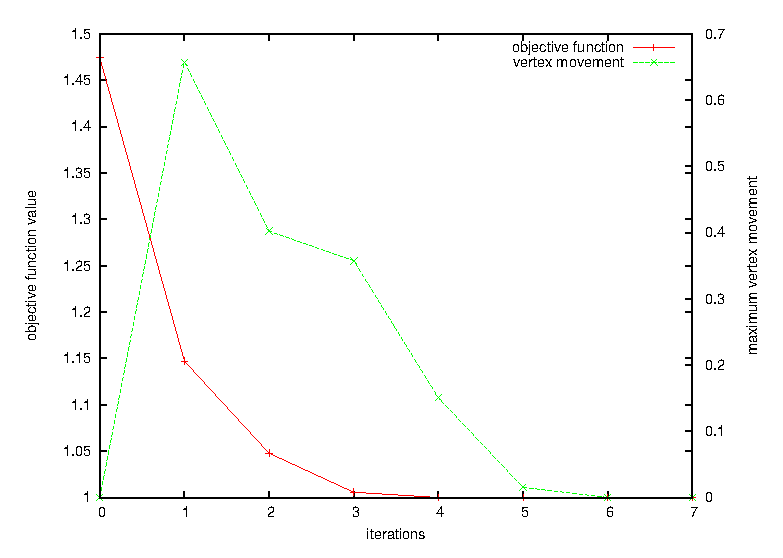
\includegraphics[width=5in]{iterplot}
\caption{\em Convergence Plot \label{fig:iterplot}}
\end{center}
\end{figure}

\section{Viewing Meshes}

VTK files read and written by the {\texttt MeshImpl} class are viewable in a plethora of visualization tools that use the VTK visualization library.

The {\texttt Mesquite::MeshWriter} namespace contains functions to export mesh in a variety of formats for visualization including:
\begin{itemize}
\item GNU Plot
\item Visualization TookKit (VTK)
\item Encapsulated PostScript (EPS)
\item Scalable Vector Graphics (SVG)
\item StereoLithography (STL)
\end{itemize}
The GNU plot format writes line data that can be used to plot a wireframe of the mesh (the mesh edges).	 Both 2D and 3D meshes can be exported in this format.	A mesh can be plotted as a 2D projection with the GNU plot command:
\begin{verbatim}
plot 'filename' with linespoints
\end{verbatim}
or as a rotatable 3D plot with the command:
\begin{verbatim}
splot 'filename' with linespoints
\end{verbatim}
Figure \ref{fig:meshgpt} is the result of plotting the mesh contained in {\texttt testSuite/higher\_order/homogeneousPart.vtk} with GNU plot.

\begin{figure}[htb!]
\begin{center}
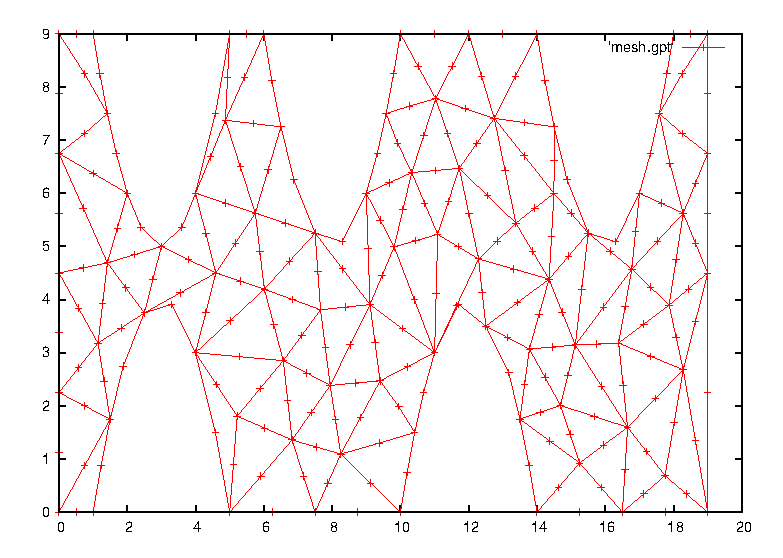
\includegraphics[width=4in]{mesh_gpt}
\caption{\em GNU Plot of 2D Quadratic Triangles \label{fig:meshgpt}}
\end{center}
\end{figure}

As mentioned in the previous section, the VTK file format can be used with a variety of visualization tools.  Figure \ref{fig:meshvtk} shows a simple plot of the same mesh in the Paraview visualization tool.

\begin{figure}[htb!]
\begin{center}
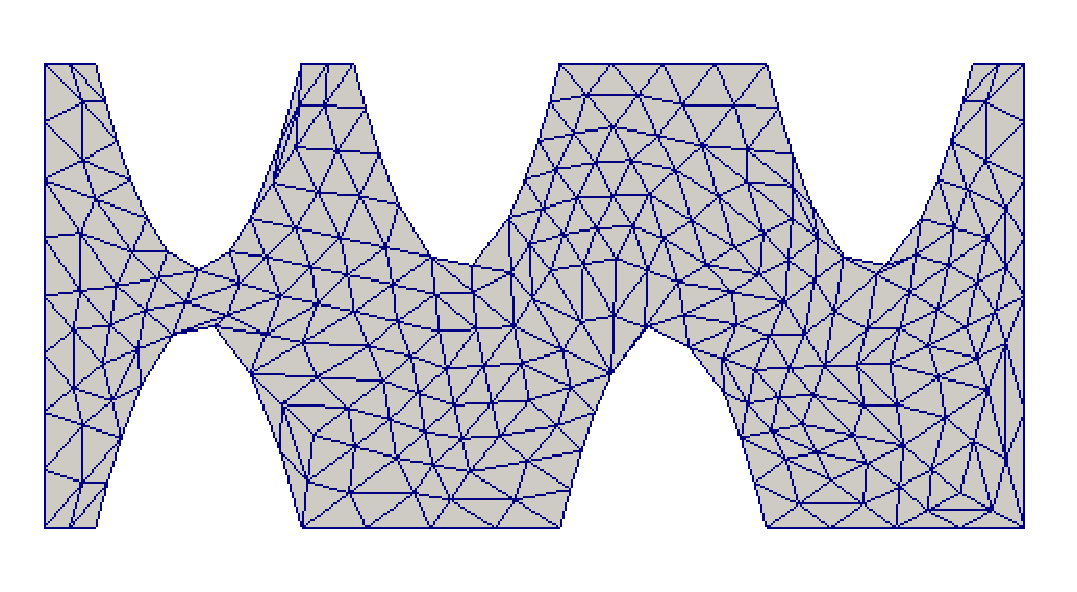
\includegraphics[width=4in]{mesh_vtk}
\caption{\em Paraview plot of 2D Quadratic Triangles \label{fig:meshvtk}}
\end{center}
\end{figure}

Figure \ref{fig:mesh} shows the output of the encapsulated PostScript writer for the mesh.  The EPS writer can write only 2D projections of the mesh.  The caller must specify a projection when calling {\texttt MeshWriter::write\_eps}.  The {\texttt testSuite/higher\_order/homogeneousPart.vtk} file contains quadratic triangle elements.  Compare the mesh edges on the mesh boundary in this plot with the output in Figures \ref{fig:meshgpt} and \ref{fig:meshvtk}.	The EPS writer in Mesquite exports the quadratic edges as curves corresponding to the classic quadratic edge shape function:
\begin{displaymath}
E(u) = \frac{1}{2}u(u-1)V_1 + (1-u^2)V_2 + \frac{1}{2}u(u+1)V_3
\end{displaymath}

\begin{figure}[htb!]
\begin{center}

\includegraphics[width=4in]{mesh}
\caption{\em Encapsulated PostScript of 2D Quadratic Triangles \label{fig:mesh}}
\end{center}
\end{figure}

The STL file format can be used to write only linear triangles.	 Higher-order triangular elements will be written as linear triangles.	An error will be returned if the mesh contains other element types.

\section{Exporting Mesh Quality}

The {\texttt QualityAssessor} class has the ability to store mesh quality values and other characteristics as tag data on mesh elements.  This data can be accessed directly by applications or written to a VTK file using the {\texttt MeshImpl} class or the applications native mesh writer (if it is capable of writing tag data.)	 The example code below was used to create the VTK file from which the Paraview plot in Figure \ref{fig:meshqual} was generated.

\begin{figure}[htb!]
\begin{center}
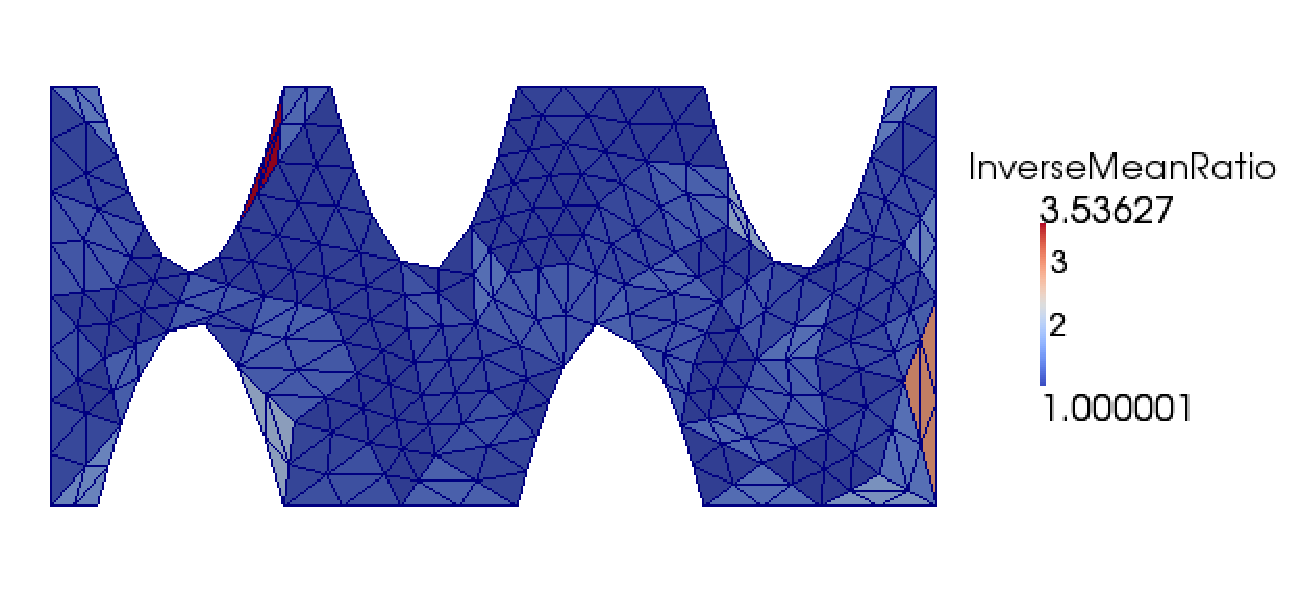
\includegraphics[width=5in]{meshqual}
\caption{\em Paraview Plot Coloring Elements by Quality Metric Value \label{fig:meshqual}}
\end{center}
\end{figure}

\newpage
\begin{samepage}
\begin{lstlisting}[frame=single]
MsqError err;
MeshImpl mesh;
mesh.read_vtk( "homogeneousPart.vtk", err );

IdealWeightInverseMeanRatio metric;
QualityAssessor qa;
qa.add_quality_assessment(&metric,0,0,0,\<"InverseMeanRatio"\>);

PlanarDomain plane(PlanarDomain::XY);
InstructionQueue queue;
queue.add_quality_assessor( &qa, err );
queue.run_instructions( &mesh, &plane, err );

mesh.write_vtk( "meshqual.vtk", err );
\end{lstlisting}
\end{samepage}

\begin{figure}[htb!]
\begin{center}
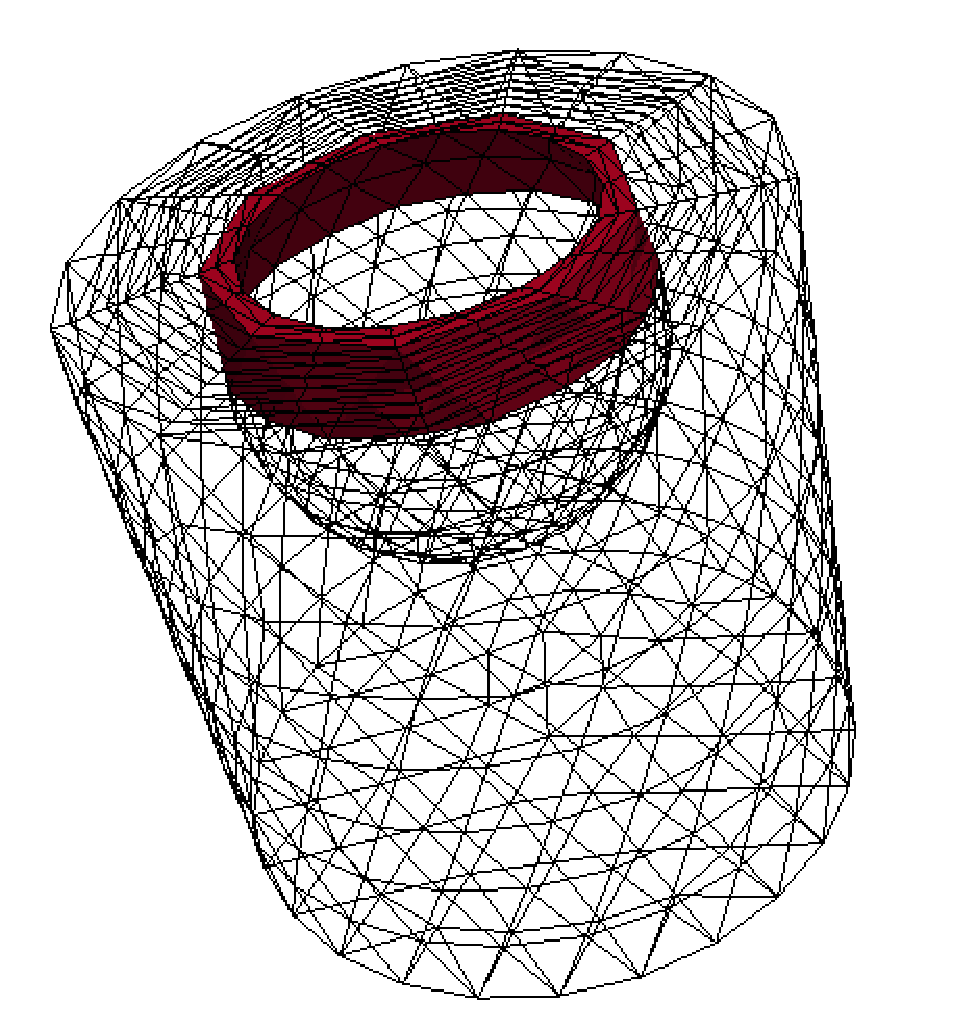
\includegraphics[width=3in]{meshqual3d}
\caption{\em Paraview Plot Showing Inverted Elements \label{fig:meshqual3d}}
\end{center}
\end{figure}

Figure \ref{fig:meshqual3d} is a Paraview plot showing the inverted elements in a quadratic tetrahedral mesh.  The mesh is plotted twice: once as a simple wireframe of the mesh boundary and a second time as solid mesh with a threshold filter on the inverted flag exported by Mesquite.  The listing below shows how the {\texttt QualityAssessor} class can be instructed to flag inverted elements:

\newpage
\begin{lstlisting}[frame=single]
MsqError err;
MeshImpl mesh;
mesh.read_vtk( "sphereCylinder_1194_inv.vtk", err );

QualityAssessor qa;
\<qa.tag_inverted_elements("Inverted");\>

InstructionQueue queue;
queue.add_quality_assessor( &qa, err );
queue.run_instructions( &mesh, &plane, err );

mesh.write_vtk( "meshqual.vtk", err );
\end{lstlisting}


\section{Mesh Optimization Visualization}

The Mesquite {\texttt TerminationCriterion} class can write the complete mesh after each iteration as either VTK or GNU Plot data suitable for viewing as an animation.	 Similar to requesting plot data as described in Section \ref {sec:optplot}, it is important to request this feature from the appropriate termination criterion instance.  If doing a global optimization, the feature should be activated for the {\em inner} termination criterion.  Otherwise the feature should almost always be activated for the {\em outer} termination criterion.

The command to request an animation of the mesh optimization in the VTK format is:
\begin{lstlisting}
tc.write_mesh_steps( "anim", TerminationCriterion::VTK );
\end{lstlisting}
This will produce a sequence of files named ``anim.1.vtk'', ``anim.2.vtk'', etc.  The files can be opened in visualization tools such as Paraview as a single set and played back as an animation.  If the optimization calculates the gradient of the objective function, that data will also be included in the file as vector data on each mesh vertex.  The components of the vector on each vertex are the partial derivatives of the objective function with respect to each coordinate value of the vertex.  A Paraview ``glyph'' filter can be used to display these vector values during the animation.


The command to request an animation of the mesh optimization in a format suitable for animating in GNU plot is:
\begin{lstlisting}
tc.write_mesh_steps( "anim", TerminationCriterion::GNUPLOT );
\end{lstlisting}
This will produce a sequence of files named ``anim.1'', ``anim.2'', etc.  It will also export a file named ``anim'' that contains the necessary GNU Plot commands to display the animation.


